% !TeX root = Report.tex

\author{
    Joar Heimonen\\
    \texttt{contact@joar.me}
    \and
    Iselin Skorpen
    \and
    Salim Said
    \and
    Mostafa Mohammadi
    \and
    Ibrar Hussain
    \and
    Hassan Ali Bokhari
}

\documentclass[12pt]{article}
% include enumitem
\usepackage{enumitem}
\usepackage{listings}
\usepackage{sectsty}
\usepackage{color}
\usepackage{float}
\restylefloat{table}
\usepackage{graphicx}
\usepackage{biblatex}

\usepackage{changepage}

\usepackage{xcolor}
\usepackage{listings}

\addbibresource{Library.bib}

\title{\textbf{Group Venus} \\ 2nd Delivery: Development Sprint}
\date{\today}

\graphicspath{ {./images/} }

\begin{document}

\subsectionfont{\fontsize{12}{14}\selectfont}

\maketitle

\pagebreak

\tableofcontents



\section{Introduction}
This report aims to document our groups experiences with the groups first design sprint.
We will be covering the following topics:

\section{Technical background}
This section aims to describe the following terms:
\subsection{Agile development\cite{AgileSoftwareDevelopment2024}}
Agile software development is software that is developed according to the ideas and values presented in the 
Manifesto for Agile Software Development\cite{ManifestoAgileSoftware}.
The manifesto presents the following core ideas:
\begin{itemize}
    \item Individuals and interactions over processes and tools
    \item Working software over comprehensive documentation
    \item Customer collaboration over contract negotiation
    \item Responding to change over following a plan
\end{itemize}
The manifesto is based on ideas created by the Agile Alliance in 2001, 
this is a group of 17 software developers.
\subsubsection{Scrum\cite{Scrum2023}}
Scrum is a type of agile methodology. The methodology was created in 1986 and widely popuralized 
after the manifesto for agile software development was published.
\subsubsection{Scrumwise\cite{scrumwiseScrumToolsScrum}}
Scrumwise is a service for managing a scrumboard. Scrumwise claims it is "The easiest Scrum tool you'll find", 
while this has not been substansiated in any meaningfull way the tool is used by many.
\subsubsection{Scrum master}
The leader of a scrum project is often refered to as the scrum master.
It is the scrum masters task to remove obstacles and streamline the teams development processes.
\subsection{Development sprint\cite{Timeboxing2024}}
A development sprint, also known as a Timebox is the process of allocating a time constraint to
reach a goal. These time constraints usually consists of a week to a month of time.
Timeboxes are great for mitigating risk as per Parkinson's law\cite{ParkinsonLaw2024}
\subsection{Backlog\cite{Backlog2022}}
A backlog usually refers to an accumulation of unfinished work.
\subsection{React\cite{React}}
React is JS\cite{ECMA262} framework for component based development of websites.
\subsubsection{Component based development\cite*{ComponentbasedSoftwareEngineering2024}}
Component based development also known as Component based software engineering is a method of software development
that aims for components of software to be loosely coupled and reusable. Component based development is an 
essential part of any agile workflow.
\subsection{Vite\cite{Vite}}
Vite is a local development server aimed at developing web applications.
\subsection{Pull Request\cite{PullRequests}}
A Pull Request is a proposal to merge one branch with another, usually from different forks of the same repository.
This project heavily relies on pull requests as this allows the scrum master to maintain the intergrity of the project.
\subsection{Burndown graph\cite{BurndownChart2024}}
A burndown graph is a graph that visualizes the remaining tasks in a backlog over time.
This graph is used as a simple status idicator during development sprints.
see \textit{Figure \ref{fig:BD}} for an illustration of a burndown graph.

\section{Sprint Goal}
We had the goal of making a functional application, with navigational options, that we could use as 
a base for the next sprint by the end of this week. \break
$\-$ The result of this week was a functional app, where you can navigate several pages. 
Certain design elements have not been implemented, but is a good base to continue our work with.

\section{Backlog}
This is the current backlog for the project, see \textit{Figure \ref{fig:BL} and \ref{fig:BL2}}.
\begin{figure}[h]
    \begin{itemize}
        \item Text input component is a work in progress.
        \item Login modal missing integration with project.
        \item Hypothetical reports on what can go wrong and access control solutions.
        \item React routing.
        \item Create Image slideshow component.
    \end{itemize}
    \caption{Our backlog}
    \label{fig:BL}
\end{figure}
\begin{figure}[h]
    \begin{adjustwidth}{-1in}{-1in}
        \centering
        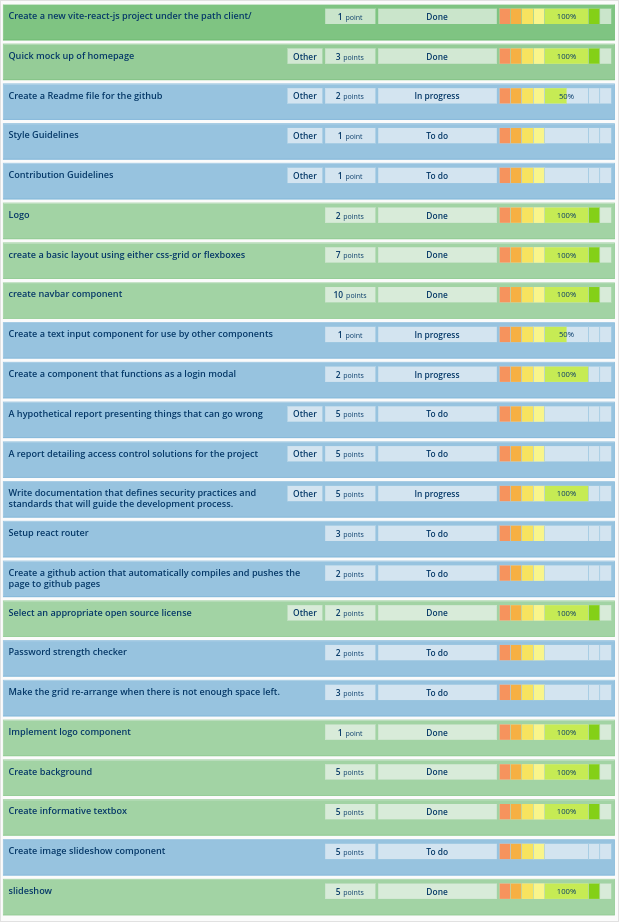
\includegraphics[scale=0.5]{backlog.png}
        \caption{An image of a scrumwise backlog}
        \label{fig:BL2}
    \end{adjustwidth}
\end{figure}
\clearpage

\section{Time}
\subsection{Participation}
This is information taken from the "Time used in this sprint" page on scrumwise.
\subsubsection{Joar Heimonen}
Joar Heimonen is the scrum master of this project.\\
Heimonen implemented the following:
    \begin{itemize}
        \item Created a Readme file for GitHub
        \item Selected an open source license
        \item Created a basic layout using either css-grid or flexboxes
        \item Created different layout components
        \item Added example pages
        \item Refactored Navigation bar
        \item Created a slideshow component
    \end{itemize}
\subsubsection{Iselin Skorpen}
Iselin made the Logo and created a mockup of the design and layout of the home page. This was to get a feel for how the website was 
going to look and function for future creation. The Navigation bar was made by Iselin. This report was also written by 
Iselin as well as Joar.
    \begin{itemize}
        \item Created a logo.
        \item Created a mockup of the home page.
        \item Created a mockup of the navigation bar.
        \item Created the Navigation bar.
    \end{itemize}
\subsubsection{Salim Said}
Salim started implementing a Text input component and a login modal. This needs integration into the application to function with everything 
else. Said also wrote a document that "defines security practices and standards that will guide the development process"\cite*{ShowitDocsSecurity}. 
This document has yet to be accepted into the main branch of the repository.
    \begin{itemize}
        \item Created a text input component.
        \item Created a Login modal.
        \item Wrote a documentation about security practices and standards for the development process.
    \end{itemize}
\subsubsection{Mostafa Mohammadi}
Mostafa Mohammadi did not show.
\subsubsection{Ibrar Hussain}
Ibrar Hussain did not show.
\subsubsection{Hassan Ali Bokhari}
Hassan Ali Bokhari created a fork of the project, and did not show for the main duration of the sprint.

\subsection{Time list}

For a picture of our time list see \textit{Figure \ref{fig:TL}}, in addition to the time list we spent about 8 hours in various meetings within the group.
\begin{figure}[h]
    \begin{adjustwidth}{-1in}{-1in}
        \centering
        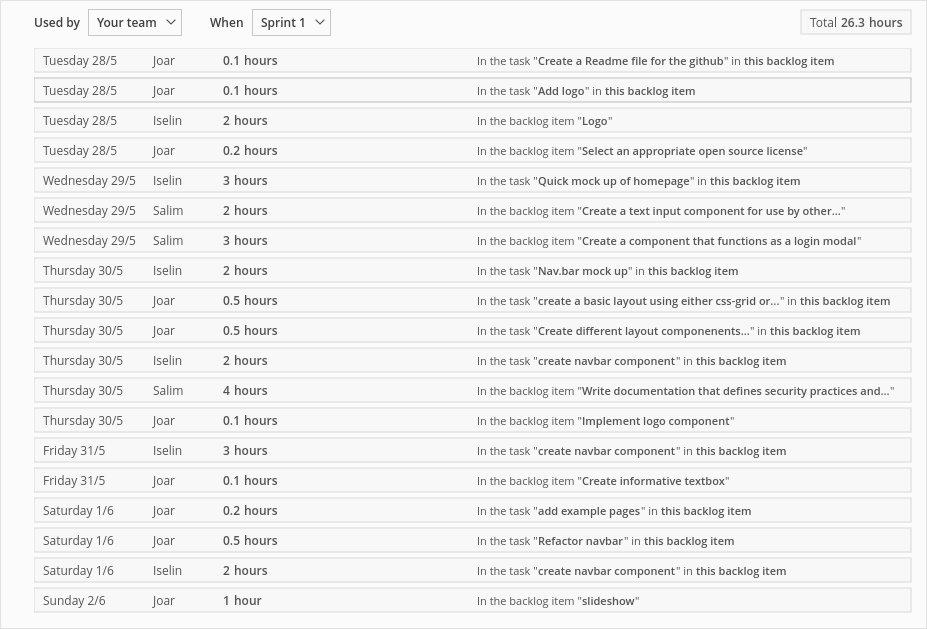
\includegraphics[scale=0.5]{timelist.png}
        \caption{An image of a scrumwise time list}
        \label{fig:TL}
    \end{adjustwidth}
\end{figure}
\clearpage
% insert picture of burndwn graph
\subsection{Burndown graph}
The burndown graph flattened out due to group members adding new tasks to the sprint as we progressed this can be seen in
\textit{Figure \ref{fig:BD}}.
\begin{figure}[h]
    \begin{adjustwidth}{-1in}{-1in}
        \centering
        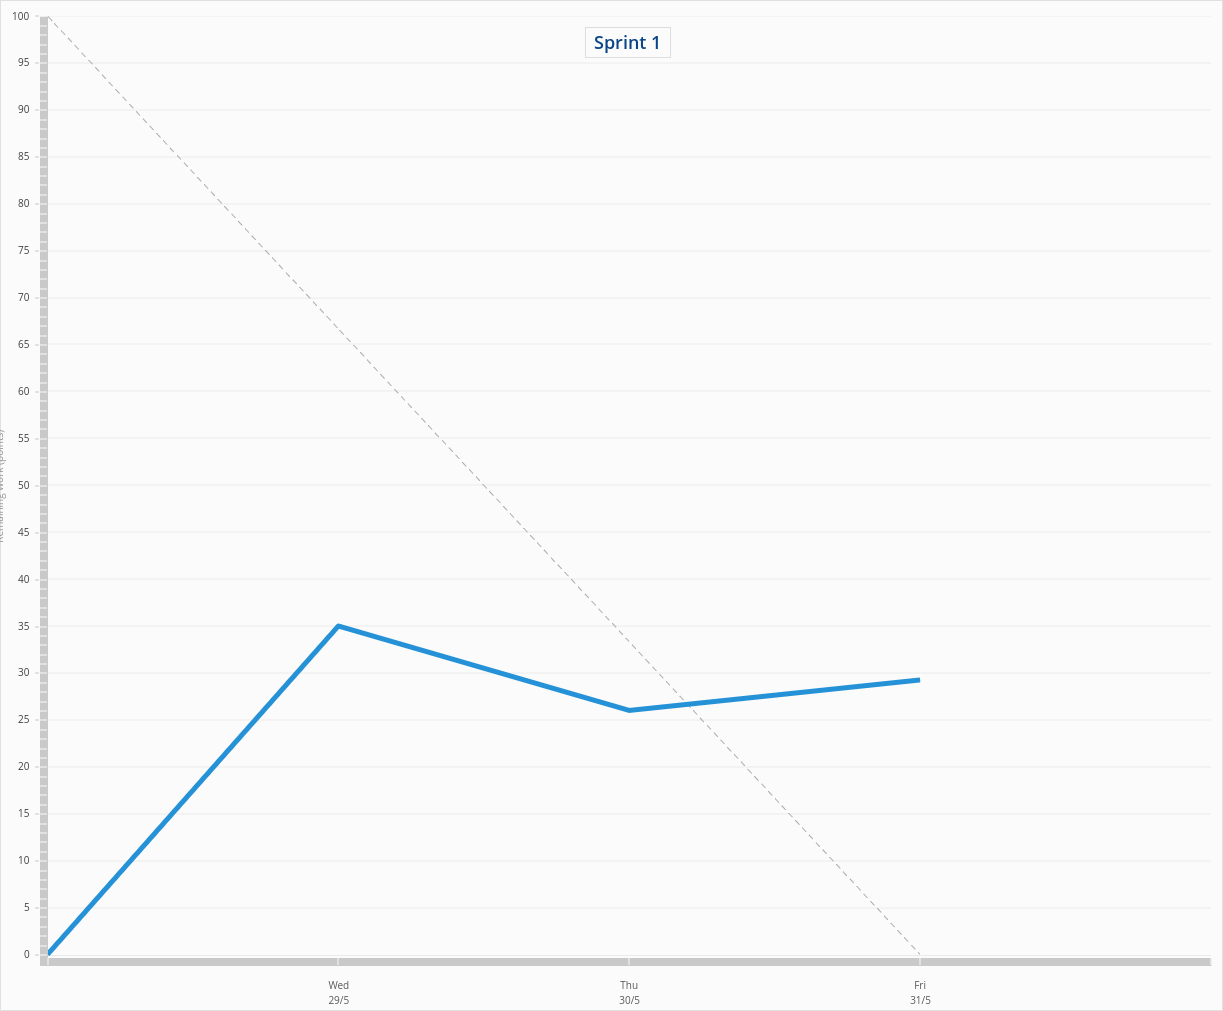
\includegraphics[scale=0.4]{burndown.png}
        \caption{An image of a scrumwise burndown graph}
        \label{fig:BD}
    \end{adjustwidth}
\end{figure}
\clearpage

\section{Reflection}
This section will anwser the following questions:
\begin{itemize}
    \item Could you have done anything differently?
    \item What were you particularly satisfied with?
\end{itemize}

\subsection{Could you have done anything differently?}
Improving our team communication and collabaration could have improved our workflow a lot. Ensuring that everyone was on the 
same page when starting production of our application. We should've had a more refined sketch done beforehand to improve 
clarity and end goal.

\subsection{What were you particularly satisfied with?}
We achieved our goal of developing a functional application, which will serve as a foundation for the next week's sprint. 
This weeks work provides us with a solid, low cost base which we can utilize to its fullest to continue our development.

\section{Notes}
It is worth noting that group participation has been lower than we expected.
Our stack was escpecially selected to allow for component based development but this was not neccesary
as the volume of Pull Requests were much lower than anticipated.

\pagebreak
\printbibliography

\end{document}